\documentclass[12pt,onecolumn]{report}
% use packages
\usepackage[utf8]{inputenc}
\usepackage{times}
\usepackage[margin=1.25in,lmargin=1.75in,footskip=.5in]{geometry}
\usepackage{ragged2e}
\usepackage{setspace}
\usepackage{graphicx}
\graphicspath{{Pics/}}
\usepackage{amsmath}
\usepackage{amssymb}
\usepackage{esint}
\usepackage{array}
\usepackage{epsfig}
\usepackage[tight,footnotesize]{subfigure}
\usepackage{multirow}
\usepackage[english]{babel}
\usepackage{csquotes}
\usepackage[backend=biber,style=ieee]{biblatex}
\usepackage{lscape}  % Useful for wide tables or figures.
\graphicspath{{Aimee_Figs/}}
\usepackage{longtable}
\usepackage{caption}
\usepackage{subfigure}
\usepackage{setspace} 
\usepackage[titletoc]{appendix}
% references/bib
\addbibresource{thesis.bib}
\setlength\bibitemsep{\baselineskip}
% numbering 
\pagenumbering{gobble}
% spacing 
\renewcommand{\baselinestretch}{1.5} % double spaced
\renewcommand{\Large}{\large}
\renewcommand{\LARGE}{\large}
\renewcommand{\huge}{\large}
\renewcommand{\Huge}{\large}
\linespread{1.5}
% enables sub-subsections in the table of contents
\setcounter{tocdepth}{3}
\setcounter{secnumdepth}{3}


\begin{document}
% title page
\centering
UNIVERSITY OF OKLAHOMA \\
GRADUATE COLLEGE \\
\vspace{5\baselineskip}
Improvements and Modeling of RFID Technology \\
\vspace{4\baselineskip}
A DISSERTATION \\
SUBMITTED TO THE GRADUATE FACULTY \\
in partial fulfillment of the requirements for the \\
Degree of \\
DOCTOR OF PHILOSOPHY\\
\vspace{5\baselineskip}
By \\
ALEXANDER MORENO \\
\setstretch{1.0}
Norman, Oklahoma \\
2020 \\

% signature page
\clearpage
~ \\ \vspace{.5in}
Improvements and Modeling of RFID Technology  \\
\vspace{2\baselineskip}
A DISSERTATION APPROVED FOR THE \\
SCHOOL OF ELECTRICAL AND COMPUTER ENGINEERING \\
\vspace{5\baselineskip}
BY \\
\vspace{6\baselineskip}
\raggedleft
\hspace*{3in}\hrulefill \\
Dr. Jessica Ruyle, Chair \\
\vspace{3\baselineskip}
\hspace*{3in}\hrulefill \\
Dr. Caleb Fulton \\
\vspace{3\baselineskip}
\hspace*{3in}\hrulefill \\
Dr. Hjalti Sigmarsson \\
\vspace{3\baselineskip}
\hspace*{3in}\hrulefill \\
Dr. Eli Bridge \\
\vspace{3\baselineskip}
\hspace*{3in}\hrulefill \\
Dr. Jay McDaniel\\


\newpage
% copyright page
\centering
\clearpage
~ \\
\vfill
\copyright~Copyright by ALEXANDER MORENO 2020 \\
All Rights Reserved.

% dedication
%\setstretch{1.6}
%\clearpage
%\vspace*{\fill}
%\textit{Dedicated to my parents, who encouraged some rather atypical dinner \\ conversations stemming from the question, ``Why?"}
%\vspace*{\fill}

\pagebreak
%\clearpage
\justify
\pagenumbering{roman}
\setcounter{page}{3}
\renewcommand{\contentsname}{Table of Contents}


% acknowledgements
\tableofcontents
%\listoftables
\listoffigures

\newpage
\begin{abstract}
\thispagestyle{plain}
\pagenumbering{roman}
\setcounter{page}{9}
\doublespacing
    [abstract stuff]
\end{abstract}

\clearpage
\pagenumbering{arabic}
\doublespacing
%%%%%%%%%%%%%%%%%%%%%%%%%%%%%%%%%%%%%%%%%%%%%%%%%%%%%%%%%%%%%%%%%%%%%%%%%%%%%
%%%%%%%%%%%   CH1: Introduction
%%%%%%%%%%%%%%%%%%%%%%%%%%%%%%%%%%%%%%%%%%%%%%%%%%%%%%%%%%%%%%%%%%%%%%%%%%%%%
\chapter{Introduction}
%%%% Motivation
    \section{Motivation}
          
% high lights of overview purpose 
As large-scale manufacturing increases, rapid identification techniques have been developed. Among these identification techniques, automatic identification (Auto-ID) procedures  has become popular in many fields of industries. Some of the most commonly used auto-ID procedures include the following but not limited to bar-code system, optical character recognition (OCR), bio-metric MM, and Radio frequency identification (RFID). This dissertation will focus on RFID technology.   

% define RFID and its gen purpose
Radio-frequency identification (RFID) technology uses electromagnetic fields to enable automatic identification of uniquely tagged objects or specimens at a distance. This technology is used to access control systems, automatic toll collection systems, vehicle tracking and immobilizers, ID and security, inventory tracking, and bio-logging. This research will focus on inventory tracking and bio-logging.

% go into details on inventory 
RFID technology is being quickly adapted into many companies' supply chains. This is due to RFID being cost-effective and providing advantages to many of the other Auto-ID procedures. Specifically, RFID technology has the advantage over bar-code and optical type systems that it does not have to be within optical line of sight.  
%RFID does not require the inventory to be in line of sight, can be obscured, and track multiple at once. % RUYLE: problematic statement
RFID systems operates in two ranges, near-field and far-field back-scatter. For the application of tracking large quantities companies will use the far-field back-scatter. The far-field back-scatter will be discussed in more detail in Section 1.2.3.  

As RFID technology continues to grow within supply chains, the tracking and identifying of various inventory needs to be taken into account. However, most RFID antennas (tags) are ``dipole-like" loops, folded dipoles, or bulky microstrip. These antennas perform poorly when applied to a metallic object. Previous work has shown an RFID antenna that is placement insensitive, no impedance change with attached to different materials \cite{ruyle2012small} \cite{ruyle2016placement}. The realized gain of this RFID tag is quite low-limiting read range \cite{ruyle2016placement}. However, it was also fund in previous work that the RFID tag couples into metallic object that is attached to\cite{moreno2016RzGain}.This dissertation will investigate how metallic object that the RFID tag is being used to track can be used strategically to increase read-range. 

% go into details on bio-logging 
Bio-logging is the data collecting of animal behavior and movement. Traditionally, the bio-logging of specimens can be a long, tedious, inaccurate, and intrusive task for researchers. Recent RFID advancements have enabled researchers to utilize RFID technology for bio-logging. RFID brings forth many benefits, such as minimal disturbance to subjects, fully automatized measurements, full-time monitoring, and inexpensive tags. However, current commercial available RFID technology for readers is expensive, not setup for animal tracking,  proprietary equipment, and difficult to apply modifications to hardware and software. Previous work by Dr. Bridge from University of Oklahoma has developed an open-source inexpensive modifiable RFID tag system. This system is called the Electronic Transponder Analysis Gateway (ETAG) Reader. This RFID system is a near-field system withe the RFID tag being passive transponder (tag). The system is a modified Arduino M0, programmable circuit board, a popular for the ease of use and available documentation. The ETAG audience do not have background in electronics or antenna design. 

%%%% REWRITE %%%
% rewrite to have stronger scientific impact 
%Therefore, this dissertation will review the background required in designing the antenna reader for a near-field RFID system, provide a software antenna design tool, and improved antenna readers via the software tool.   

%
%%%% Overview of RFID    
    \section{Overview of RFID}
        \subsection{Core Components of RFID System}
            
An RFID system is composed of three components:
\begin{itemize}
    \item A transponder (tag), consists of antenna, chip, and sometimes a battery. It is the data-carrying device.
    \item An interrogator (the reader/write device), consists of reader antenna, radio-frequency electronics, and control module
    \item A controller (host electronic or computer), consists of database 
\end{itemize}


\begin{figure}[htp]
    \centering
    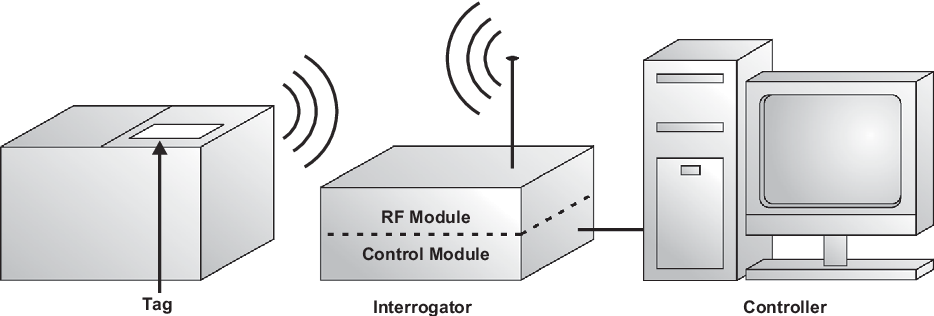
\includegraphics[scale=0.45]{Figs/RFID_Blocks.png}
    \caption{The basic components to an RFID system. \cite{laran2004basic}}
    \label{fig:RFIDBlocks}
\end{figure}


Some RFID systems can have the interrogator and the controller be one component. The simple interaction between these components is that the tag and interrogator communicate information between each other via radio-frequency (RF) waves. This interaction occurs when the tagged specimen enters the read zone of the interrogator, retrieves information from the tag. The information that tags can store can be serial numbers, time stamps,  or other useful data. Once the interrogator retrieves the tag's information the controller can implement another procedure such as recording inventory, granting access, active another electronic such as a motor, etc. 

The RFID tags fall into two categories, passive and active transponders. Passive RFID tags do not have on-board power supply instead they obtain their power from the interrogator's transmitted signal (magnetic or electromagnetic field). The tag transmits its data via modulation (e.g. by load modulation or modulated back-scatter). In most cases, passive tags are smaller and less expensive than active tags. Active tags contain an on-board power supply, such as a battery or solar cell, to provide voltage to the chip. The active tags can generate their own fields and modulation thus increasing the read-range between the transponder and the interrogator. Important to note that active tags are typically not able to generate high-frequency signals alone, can only modulate the fields from the interrogator.    
Tags can also be categorized as read-only (RO) and read/write (RW). The RO tags can only be read. Once these RO tags are fabricated their data can be altered. Typically used for static information such as part numbers, ID, serial numbers, etc. The RW provides more flexibility such as allowing the data to be changed, storing much more information than RO tags, and easy accessibility.   


        \subsection{Near-Field Based RFID Design}
            RFID systems that operating at the High Frequency (HF) band or lower use near-field based RFID design. The overall RFID system is electrically small that RFID reader antenna's load can be modulated. This is accomplished via near-field coupling between reader and tag and can be described in terms of Faraday's principle of magnetic induction. The reader tag has a alternating current pass through the coiled antenna that generates a magnetic field. When the RFID tag is within the reader's magnetic fields, resulting in an induced current within the RFID tag. This induced current yields a voltage across the tag, the tag has a minimal voltage requirement to turn it on. Once the tag turns on, it will generate its own magnetic fields to send data back to the RFID reader. The tag's load is applied to the reader's coiled antenna over time, causing a modulation. The RFID reader can encode this modulation into data.   

\begin{figure}[htp]
    \centering
    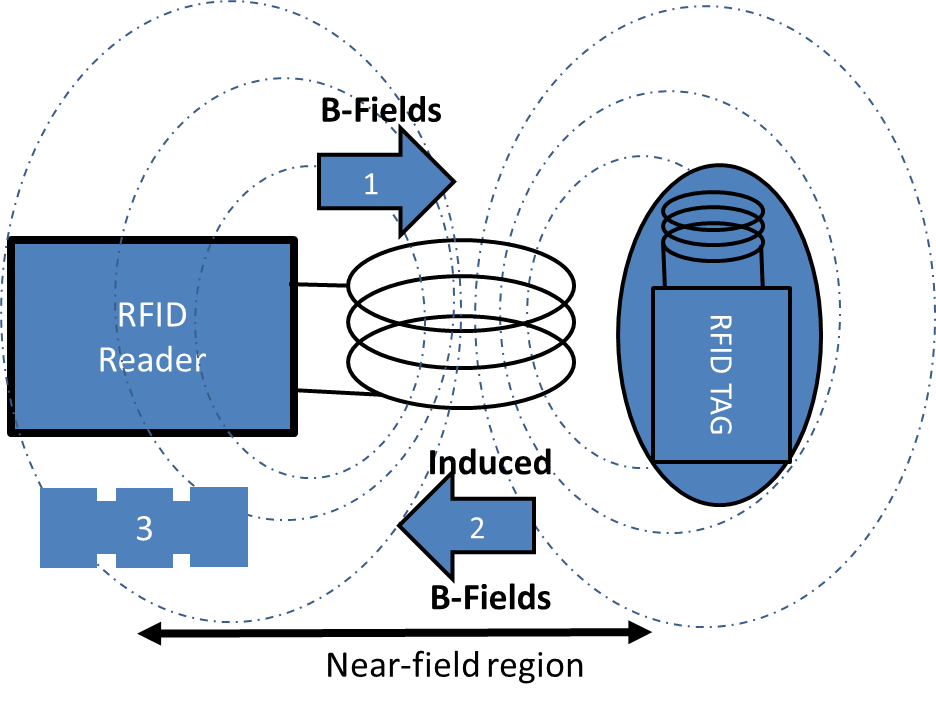
\includegraphics[scale=0.6]{Figs/nearField.png}
    \caption{Near-field power/communication set up RFID system. 1) RFID Reader creates B-Fields. 2) Reader B-Fields turns on tag, tag generates its own B-Field. 3) Tag's B-Field scatters into RFID Reader, encodes the modulation into data.}
    \label{fig:RFIDBlocks}
\end{figure}


%As previously mentioned the tag transmits its data via modulation. The two modulations are load modulation or modulated back-scatter. The load modulation uses the near-field coupling between reader and tag, can be describe via Faraday's principle. An alternating current is passed through the reader's (coiled) antenna, generating a magnetic field. Once the RFID tag is placed within the reader's fields this will result in an induced alternating voltage across the tag. This voltage will be used within the tag to turn its chip. Once the chip has been successfully activated, the tag yields its own magnetic fields that interact with the reader. The tag's load is applied to the reader's coiled antenna over time, causing a modulation. Typically load modulations operating under 100MHz (LF and HF).


        \subsection{Far-Field Based RFID Design}
            This modulation can be encoded to retrieve the tag's data. The modulated back-scatter (or far-field coupling) retrieves the electromagnetic waves from the tag's antenna when not within the near-fields. These tags are typically designed for a frequency band such that there is a mismatch causing energy to be reflected back to the reader. The tag's impedance can be changed over-time to cause modulation, this modulation can be encoded by the reader to obtain the tag's data. Typically modulated back-scatter operates within the UHF frequency band. 

\begin{figure}[htp]
    \centering
    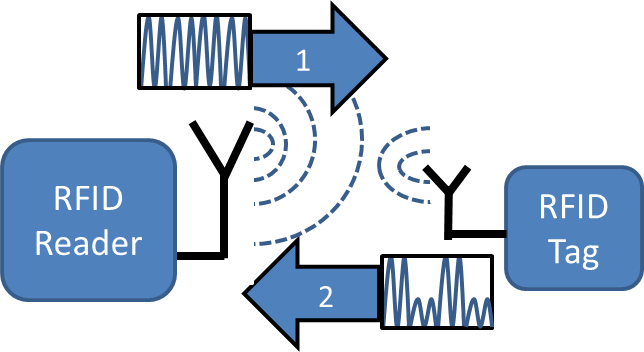
\includegraphics[scale=1.2]{Figs/FF_BS.png}
    \caption{Far-field power/communication set up RFID system. 1) RFID Reader transmits an emf 2) RFID Tag modulates and scatters the RFID Reader's emf 3) RFID Reader encodes the back-scatter signal from RFID Tag.}
    \label{fig:RFIDBlocks}
\end{figure}
        \subsection{Modulation Techniques}
            A brief mentioned two basic modulation techniques used within RFID is amplitude shift keying (ASK) and binary phase-shift keying (BPSK). ASK represents digital data as variations in the amplitude of a carrier wave. The binary symbol 1 is represented as a duration of T seconds at a fixed-amplitude and binary symbol is for all other cases that are not that fixed-amplitude. BPSK (or PRK or 2PSK), a form of phase-shift keying, is a two-phase modulation scheme. The signal has two different phase states in the carrier signal, $\theta=0^\circ$ (binary 1) and $\theta=180^\circ$ (binary 0). In Figure [] shows an example of these two modulation schemes.
\newline
I need to input a figure
%%%% Research Objetives            
    \section{Research Objectives}
        The research objectives are separated into two projects. Project one, the biological research's research objective is to provide a simple implementation to design multi-coiled wire antennas that yields a higher read-range and inductance for near-field RFID systems. This tool will decrease development time of fabrication of the multi-coiled wire antennas, provide an insight of multi-coiled wire antenna designs, and provide alternate design suggestions for improved read-range.  

Project two is to optimize RFID tag's coupling based on orientation and position placement upon a canonical metallic object's current distribution to increase modulated far-field back-scatter (read-range). %This dissertation will report its findings, provide design guidelines, and  

% The research objectives are separated into two projects. The first project as previously discussed involves bio-logging using an inexpensive open-source RFID tag system. The objectives is to create a GUI software tool to enable non-antenna engineers to rapidly prototype multi-coiled wire antennas for LF and HF frequencies bands, provide design improvements, provide a software user guide, and instructions on the construction of multi-coiled wire antennas. The second project involves the investigation of impact on modulated back-scattering of metallic object with placement of RFID tag. This investigation will report the findings that include bounds in which the modulated back-scattering is impacted upon RFID tag's placement, those effects upon modulated back-scattering, and recommend placement of the tag on the metallic object.   
%%%% Disseration Outline
    \section{Dissertation Outline}
        Chapter 2 discusses the details of first project and will involve the following overview of method of moments and characteristics mode analysis, background of insensitive placement RFID Tag, and investigation of canonical metallic backing upon insensitive placement RFID tag.  Chapter 3 discusses the details of the software tool that constructs multi-coiled wire antenna, generate the  magnetic fields, read-range, and inductance. The final chapter will summarize, addressed this dissertation's scientific impact, and future work. 
        
%%%%%%%%%%%%%%%%%%%%%%%%%%%%%%%%%%%%%%%%%%%%%%%%%%%%%%%%%%%%%%%%%%%%%%%%%%%%%
%%%%%%%%%%%   CH2: Investigation of Canonical Metallic Backing Upon  Insensitive Placement RFID Tag
%%%%%%%%%%%%%%%%%%%%%%%%%%%%%%%%%%%%%%%%%%%%%%%%%%%%%%%%%%%%%%%%%%%%%%%%%%%%%   
\chapter{Investigation of Canonical Metallic Backing Upon  Insensitive Placement RFID Tag}
%%%%% Introduction
    \section{Introduction}
%%%%% MOM    
    \section{Overview of Method of Moments and Characteristics Mode Analysis}
        \subsection{Method of Moments}
        \subsection{Characteristics Mode Analysis}
%%%% Background of Placement Insensitive  RFID Tag     
    \section{Background of Placement Insensitive  RFID Tag}
        \subsection{Background}
        \subsection{Input Impedance}
        \subsection{Realized Gain}
        \subsection{Far-Field Back-Scatter}
            % \subsubsection{}
    %\section{Investigation of  Metallic Plate Upon  Insensitive Placement RFID Tag}
%%%% Impact of Placement of RFID Tag on Metallic Plate
    \section{Impact of Placement of RFID Tag on Metallic Plate}
        \subsection{Applying CMA to Metallic Plate}
        \subsection{Realized Gain for RFID Tag Placed on Metallic Plate}
            \subsubsection{Simulation Results}
        \subsection{Far-Field Back-Scattering for RFID Tag Placed on Metallic Plate}
            \subsubsection{Simulation Results}
            \subsubsection{Measured Results}
%    \section{Investigation of  Metallic Cuboid Upon  Insensitive Placement RFID Tag}    
%%%% Impact of Placement of RFID Tag on Metallic Cuboid
    \section{Impact of Placement of RFID Tag on Metallic Cuboid}
        \subsection{Applying CMA to Metallic Cuboid}
        \subsection{Realized Gain for RFID Tag Placed on Metallic Cuboid}
            \subsubsection{Simulation Results}
        \subsection{Far-Field Back-Scattering for for RFID Tag Placed on Metallic Cuboid}
            \subsubsection{Simulation Results}
%%% Conclusions
    \section{Conclusions}
%%% Future Work
    \section{Future Work}
    
%%%%%%%%%%%%%%%%%%%%%%%%%%%%%%%%%%%%%%%%%%%%%%%%%%%%%%%%%%%%%%%%%%%%%%%%%%%%%
%%%%%%%%%%%   CH2: RFID Applications for Biological Research
%%%%%%%%%%%%%%%%%%%%%%%%%%%%%%%%%%%%%%%%%%%%%%%%%%%%%%%%%%%%%%%%%%%%%%%%%%%%% 
\chapter{RFID Applications for Biological Research}
%%%% Introduction
    \section{Introduction}
        \include{CH1_Intro/1.0_Introduction}
%%%% Modeling Wire Antennas
    \section{Modeling Wire Antennas}
        \subsection{Overview of Biot-Savart Law and Applications}
        \subsection{Overview of Mutual Inductance}
        \subsection{Implementation Read-Range Modeling} 
%%%% Constriction of Multi-Coiled Wire Antennas
    \section{Construction of Multi-Coiled Wire Antennas}
        \subsection{Elliptical Multi-Coiled Wire Antennas}
        \subsection{Rectangular Multi-Coiled Wire Antennas}
%%%% Test Setup    
    \section{Test Setup}
%%%% Measurements Results
    \section{Measurements Results}
%%%% Software Application    
    \section{Software Application}
%%%% Software User GUide
    \section{Software User Guide} 
%%%% Conclusions
    \section{Conclusions}
%%%% Future Work
    \section{Future Work}
    
%%%%%%%%%%%%%%%%%%%%%%%%%%%%%%%%%%%%%%%%%%%%%%%%%%%%%%%%%%%%%%%%%%%%%%%%%%%%%
%%%%%%%%%%%   CH4: Conclusion, Scientific Impact, and Future Work
%%%%%%%%%%%%%%%%%%%%%%%%%%%%%%%%%%%%%%%%%%%%%%%%%%%%%%%%%%%%%%%%%%%%%%%%%%%%%     
\chapter{Conclusions, Scientific Impact, and Future Work}
%%%% Summary    
    \section{Summary}
%%%% Scientific Impact
    \section{Scientific Impact}
%%%% Future Work    
    \section{Future Work}
%%%%%%%%%%%%%%%%%%%%%%%%%%
%%%%%%%%%%%%%%%%%%%%%%%%%%

\clearpage
\setstretch{1.0}
\nocite{*}
\printbibliography
%\bibliographystyle{IEEEtran}
%\bibliography{thesis}

% Any appendices will go here
\begin{appendices}

\chapter{Fabrication Process} \label{Fabrication}
% \subfile{Chapters/App1}

\setstretch{1.0}
\chapter{List of Acronyms and Abbreviations}
% \subfile{Chapters/App2}

\chapter{Summary of Contributions}
% \subfile{Chapters/App3}

\chapter{}

\end{appendices}


\end{document}

